\chapter{Research Context: Statistical Learning and Visual Analytics of Building Data}
\label{sec:litreview}

% \color{green} insert a long introduction as to why unsupervised techniques and visual analytics are necessary to this thesis}
This section gives an extensive overview of the techniques developed to extract automatically information from raw data to meet the scalability challenge. This content is developed as a publication submitted to the Renewable and Sustainable Energy Reviews Journal \citep{miller_review_????}. The domains and range of techniques reviewed go beyond the scope of this dissertation. It considers a range of applications and objectives beyond the presented framework and research questions. The purpose of this effort is to set a wider context for understanding and discuss broader challenges and opportunities.

Researchers from several domains have developed methods of extracting insight from raw data from the built environment. Often these methods fall into the category of statistical learning, often from unsupervised learning. Methods from this sub-domain of machine learning are advantageous due to their ability to characterize measured or simulated performance data quickly with less analyst intervention, meta-data, and ground truth labeled data. In this section, a review of previous work in analytics methods is covered by the categories of smart meter analytics, portfolio analytics, operations and control, and anomaly detection for buildings.

\section{Previous Reviews of Data Analytics in Buildings}
\label{sec:previousreviews}

Various reviews have been completed that overlap with this section. Most of them are designed to focus on a single core domain of research; the main two areas are building operations analysis and smart grid optimization. One of the earliest reviews of artificial intelligence techniques for buildings was completed in 2003 by Krarti and covered both supervised and unsupervised methods \citep{krarti_overview_2003}. Dounis updated this work and focused on outlining specific techniques in detail \citep{dounis_artificial_2010}.  Reddy's seminal book about a large variety of analysis techniques for energy engineers includes chapters on clustering and unsupervised methods specifically \citep{reddy_applied_2011}. Lee et al. describe a variety of retrofit analysis toolkits which incorporate unsupervised and visual analytics approaches in a practical sense \citep{lee_energy_2015}. Ioannidis et al. created a large ontology of data mining and visual analytics for building performance analysis, however with a strong focus on the techniques and not examples of works using them \citep{ioannidis_big_2015}. From the utility and power grid side, Morias et al. created a general overview of various data mining techniques as focused on power distribution systems \citep{morais_overview_2009}. Chicco covered clustering methods specifically focused on load profiling tasks \citep{chicco_overview_2012}. Zhou et al. included the concept of customer load classification  \citep{zhou_review_2013}.\\

\section{Overview of Publications}
\label{Overview}
The work for this section was created through a selection of unsupervised analytics categories outlined by authoritative sources from the machine learning community \citep{hastie_elements_2009,james_introduction_2013,duda_pattern_2012,mirkin_clustering:_2012}. The groups selected are clustering, novelty detection, motif and discord detection, and rule extraction. The field of visual analytics was added to these groups to cover the presentation layer of many of these types of techniques. An initial search of publications was then selected for inclusion through a Google Scholar search of the combination of the method categories and the terms ``building energy'', ``building performance analysis'', and ``building energy analysis''. From this initial list of publications, a set of application categories and sub-categories was developed as seen in Figure \ref{fig:categoriespie}. A more detailed search of each application class was then completed to account for the unique analytics techniques used in those domains. Only publications with a majority of the focus on utilization of unsupervised techniques and with a focus only on non-residential buildings are reviewed. Only works completed since 2005 are included to discuss only the most contemporary work and due to the relatively recent development of most of the techniques examined. A cutoff date of April 1, 2016, is applied for inclusions of publications in this review.

\begin{figure}[ht!]
\begin{center}
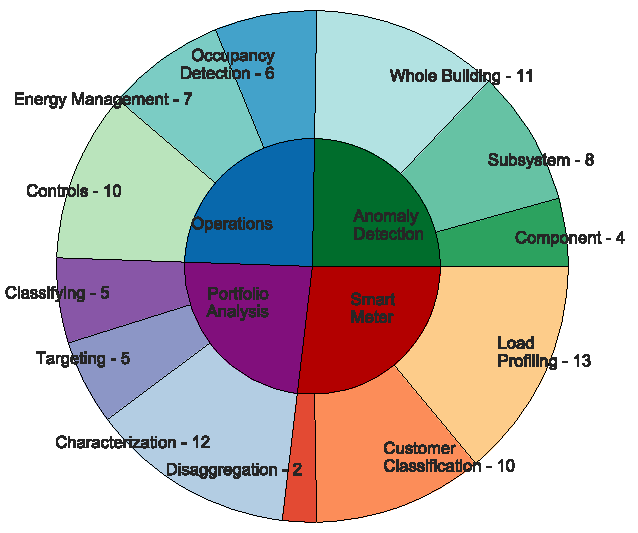
\includegraphics[width=0.7\columnwidth]{figures/PieChart_resized/PieChart_resized}
\caption{Categories and sub-categories (including number of publications) of building performance analysis applications of statistical learning and visual analytics
\label{fig:categoriespie}%
}
\end{center}
\end{figure}

\subsection{Research Sectors}
\label{sec:subsectors}

Figure \ref{fig:yearbreakdown} illustrates the breakdown of publications based on the year published since 2005. They are further divided into four broad research domains: building energy analysis, building simulation, computer science and electrical engineering. These research field categories were subjectively determined for each paper through evaluating a combination of which university department the authors were from and in which publication the study was published. Building energy analysis pertains to researchers who predominantly focus on measured data analysis from buildings while simulation experts research forward modeling and simulation of building and urban systems. Both fields of study most often exist within architecture or mechanical engineering departments. Electrical engineering and computer science are two well-established domains and exist in their departments. It is noticed that there is a gradual increase in the number of publications over the last ten years with electrical engineering and building energy analysis being the most common in the first few years and computer science and building simulation picking up since 2008. 

\begin{figure}[ht!]
\begin{center}
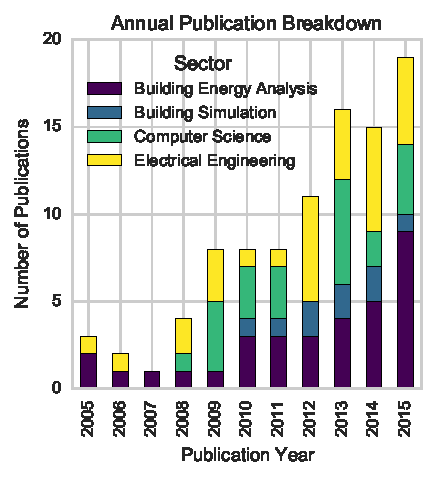
\includegraphics[width=0.5599999999999999\columnwidth]{figures/PublicationYear/PublicationYear}
\caption{Breakdown of publications by year published and research domain
\label{fig:yearbreakdown}%
}
\end{center}
\end{figure}

\subsection{Publications Venues}
This section analyzes the prevalence of certain publication venues within this section. Figure \ref{fig:journalbreakdown} illustrates the breakdown of the publication venues represented. The Energy and Buildings Journal from the building energy analysis domain dominates this list with 17 articles. Building simulation and energy analysis research domains publish most often in this journal as well as Applied Energy and Energy Efficiency. Several IEEE conferences and journals are also dominant as most of the papers from the electrical engineering domain are in these venues.

\begin{figure}[ht!]
\begin{center}
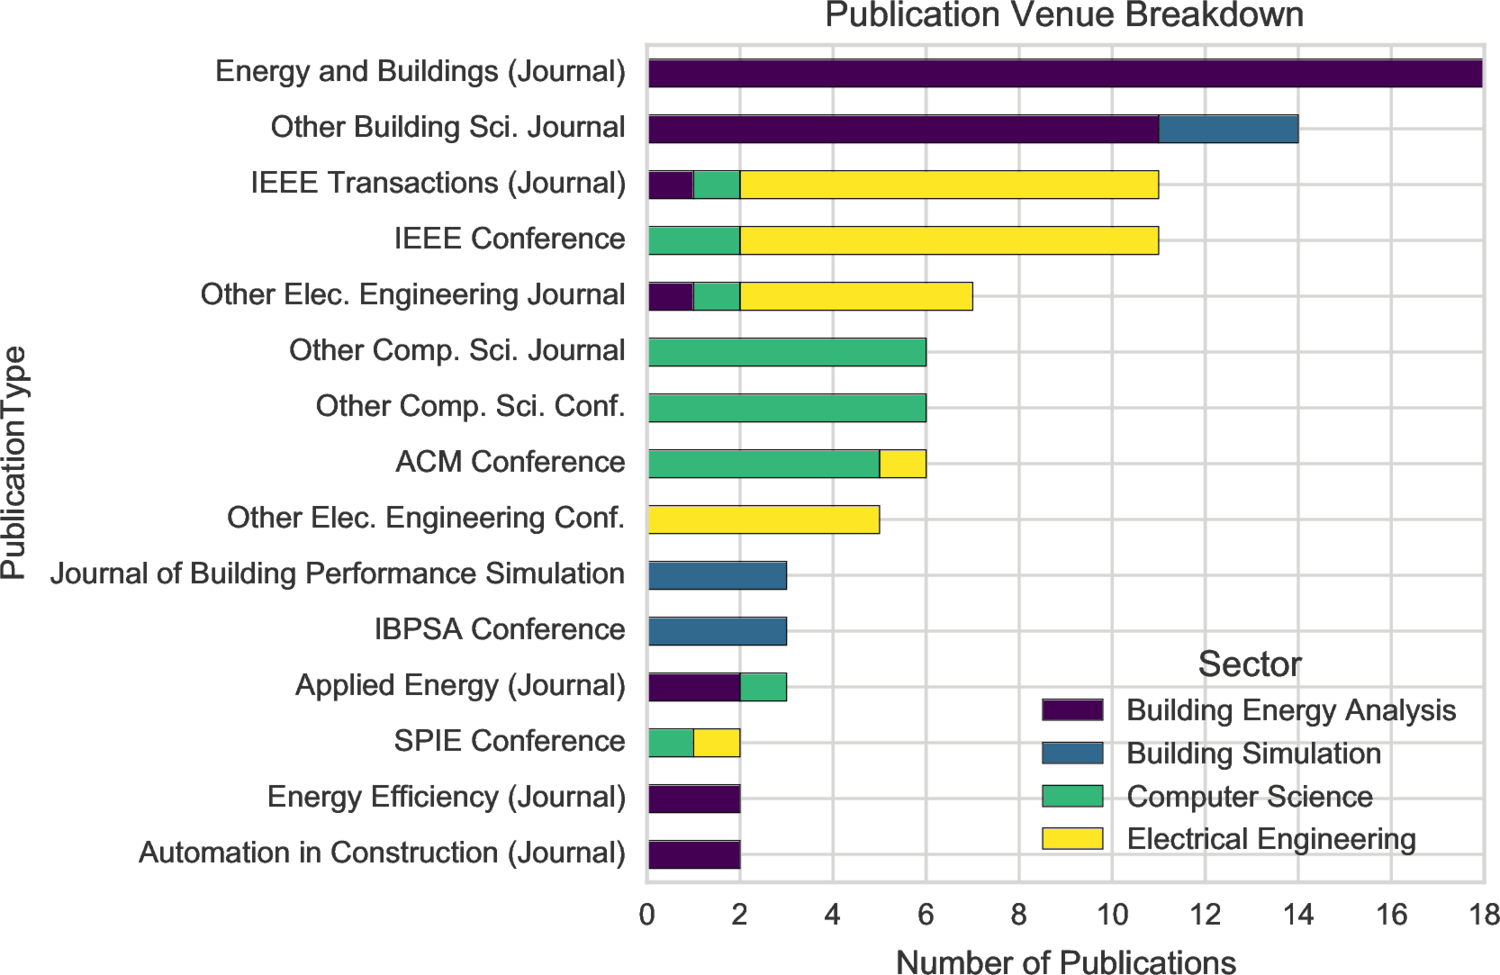
\includegraphics[width=1\columnwidth]{figures/PublicationVenues/PublicationVenues}
\caption{Breakdown of publications by publication type and research domain
\label{fig:journalbreakdown}%
}
\end{center}
\end{figure}

\section{Smart Meter Analytics}
\label{SmartMeter}
Advanced Metering Infrastructure (AMI), also known as smart meter systems, is a network of energy meters, most often focused on the electrical power measurement of a whole building. These systems are implemented and utilized by electrical utility providers. Conventional metering infrastructure only facilitates monthly data collection for billing purposes, while the new AMI framework allows for sub-hourly electrical demand readings. These data are primarily used for demand characterization and billing, however, many additional uses are being discovered. A wide-range of studies have been completed in recent years to focus on a range of issues related to automatically extracting information from these data using unsupervised techniques. In this section, three sub-categories of application are discussed: load profiling, account classification, and disaggregation.

\subsection{Load Profiling}
Load profiling is the process of grouping temporal subsequences of measured energy data for the purpose of characterizing the typical behavior of an individual customer. It involves time-series clustering and feature extraction. Chicco et al. provide an original example in our review of this process using support vector machine clustering \citep{chicco_support_2009}. Gullo et al. and R\"as\"anen et al. took the process further by introducing a framework of various clustering procedures that were implemented on case studies \citep{gullo_low-voltage_2009,rasanen_feature-based_2009}. Ramos et al., Iglesias et al., and Panapakidis et al. tested various conventional and new clustering methods and similarity metrics to determine those most applicable to electrical load profiling \citep{iglesias_analysis_2013,ramos_typical_2012,panapakidis_evaluation_2015}. Chicco et al. explored new clustering techniques based on ant colony grouping while Pan et al. discovered the use of kernel PCA for the same purpose \citep{chicco_electrical_2013,pan_kernel-based_2015}. Several groups of researchers such as Lavin and Klabjan and Green et al. have found efficient use in using the core K-Means clustering algorithm for load profiling \citep{lavin_clustering_2014,green_divide_2014}. Shahzadeh et al. discussed the use of profiling as applied to forecast accuracy of temporal data \citep{shahzadeh_improving_2015}. Two studies diverge from the standard profile development using clustering paradigm. The first is by De Silva et al. who uses Incremental Summarization and Pattern Characterization (ISPC) instead of clustering to find load profiles \citep{de_silva_data_2011}. The other is the visual analytics-based approach of creating a smart meter analytics dashboard by Nezhad et al. to set up and inspect typical load profiles \citep{jarrah_nezhad_smartd:_2014}.

\subsection{Customer Classification}
Automated account classification is the next sub-category that utilizes unsupervised learning techniques within the smart meter domain. These methods often employ load profile clustering as a first step but differentiate themselves in using those features to classify accounts, or buildings, that fit within various categories. Therefore, account classification is a type of manual semi-supervised analysis utilizing load profiling as a basis. The study by Figueiredo et al. harnessed K-Means and a labeled sample from accounts in Portugal to showcase this concept \citep{figueiredo_electric_2005}. Verdu et al. and R\"as\"anen et al. applied self-organizing maps (SOM) to accomplish a similar study that classifies accounts according to the applicability of several demand response scenarios \citep{verdu_classification_2006,rasanen_reducing_2008}. Vale et al. give an overview of a general data mining framework focused on characterizing customers \citep{vale_data_2009}. Florita et al. diverge from the use of measured data by creating a massive amount of simulation data of load profiles to quantify energy storage applications for the power grid \citep{florita_classification_2012}. Fagiani et al. use Markov Model novelty detection to automatically classify customers who potentially have leakage or waste issues \citep{fagiani_novelty_2015}. Cakmak et al. and Liu et al. test new visual analytics techniques within more holistic analysis framework for analyzing customers \citep{cakmak_new_2014,liu_smas:_2015}. Borgeson used various clustering and occupancy detection techniques to analyze a large AMI data set from California \citep{borgeson_targeted_2013}. Bidoki et al. tested various clustering techniques to evaluate applicability for customer classification \citep{bidoki_evaluating_2010}. A recent study in Korea develops a new clustering method for segmenting customers to analyze demand response incentives \citep{jang_variability_2016}.

\subsection{Disaggregation}
The last area of smart meter data analysis is the field of meter disaggregation. Disaggregation attempts decompose a measurement signal from a high level reading to the individual loads being measured. This domain is well-researched from a supervised model perspective but recent attempts at unsupervised, pattern-based disaggregation were developed to facilitate implementation on unlabeled smart meter data. Shao et al. use Dirichlet Process Gaussian Mixture Models to find and disaggregate patterns in sub-hourly meter data \citep{shao_temporal_2013}. Reinhardt and Koessler use a version of symbolic aggregate approximation (SAX) to extract and identify disaggregated patterns for the purpose of prediction \citep{reinhardt_powersax:_2014}. These studies are also unique in that few of the disaggregation studies focus on commercial buildings as opposed to residential buildings.

\section{Portfolio Analytics}
\label{PortfolioAnalytics}

Portfolio analysis is a domain in which a large group of buildings, often located in the same geographical area or owned or managed by the same entity, are analyzed for the purpose of managing or optimizing the group as a whole. Each subsection covers the publications reviewed in this domain that fall into three categories: characterization, classification, and targeting.

\subsection{Characterization}
Publications that address the characterization of a portfolio of buildings include unsupervised techniques meant to evaluate and visualize the range of behaviors and performance of the group. A majority of the techniques utilized are either clustering or visual analytics that provide a model of exploratory analysis that enable further steps. Seem produced an influential study that extracts days of the week with similar consumption profiles \citep{seem_pattern_2005}. Further clustering work was completed by An et al. to estimate thermal parameters of a portfolio of buildings \citep{an_estimation_2012}. Lam et al. used Principal Component Analysis to extract information about a group of office buildings \citep{lam_principal_2008}. Approaches focused on visual analytics and dashboards were completed by Agarwal et al., Lehrer, and Lehrer and Vasudev \citep{agarwal_energy_2009,lehrer_research_2009,lehrer_visualizing_2011}. Granderson et al. completed a case study-based evaluation of energy information systems, in which some methods combine some unsupervised approaches with visualization \citep{granderson_building_2010}. Diong et al. completed a case study as well focused on a specific energy information system implementation  \citep{diong_establishing_2015}. Mor\'an et al. and Georgescu and Mezic developed hybrid methods that employed visual continuous maps and Koopman Operator methods respectively to visualize portfolio consumption\citep{moran_analysis_2013,georgescu_site-level_2014}. Miller et al. completed two studies focused on the use of screening techniques to automatically extract diurnal patterns from performance data and use those patterns to characterize the consumption of a portfolio of buildings  \citep{miller_forensically_2015,miller_automated_2015}. Yarbrogh et al. used visual analytics techniques to analyze peak demand on a university campus \citep{yarbrough_visualizing_2015}.

\subsection{Classification}
The concept of classifying buildings within a portfolio supplements the characterization techniques by assigning individual buildings to subgroups of relative performance for the purpose of benchmarking or decision-making. Santamouris et al. produced a report using clustering and classification to assign schools in Greece to subgroups of similar performance \citep{santamouris_using_2007}. Nikolaou et al. and Pieri et al. further extended this type of work to office buildings and hotels\citep{nikolaou_application_2012,pieri_identifying_2015}. Heidarinejad et al. released an analysis of clustered simulation data to classify LEED-certified office buildings \citep{heidarinejad_cluster_2014}. Ploennigs et al. created a platform for monitoring, diagnosing and classifying buildings and operational behavior within a portfolio to quickly visualizing the outputs \citep{ploennigs_e2-diagnoser:_2014}.

\subsection{Targeting}
Targeting is a concept that builds upon characterization and classification to identify specific buildings or measures to be implemented in a portfolio to improve performance. These publications are differentiated in that specific measures are identified in the analysis. Sedano et al. use Cooperative Maximum-Likelihood amongst other techniques to evaluate the thermal insulation performance of buildings \citep{sedano_improving_2009}. Gaitani et al. used PCA and clustering to target heating efficiency in school buildings \citep{gaitani_using_2010}. Bellala et al. used various methods to find lighting energy savings on a campus of a large organization \citep{bellala_towards_2011}. Petcharat et al. also found lighting energy savings in a group of buildings \citep{petcharat_assessment_2012}. Cabrera and Zareipour used data association rules to complete a similar study to find wasteful patterns \citep{cabrera_data_2013}. Geyer et al.  and Schlueter et al. test various clustering strategies to group different buildings within a Swiss alpine village according to their applicability for retrofit interventions \citep{geyer_application_2016} and thermal micro-grid feasibility \citep{schlueter_analysis_2016}.

\section{Operations, Optimization, and Controls}
\label{Operations}
Unsupervised techniques focused on individual buildings themselves are placed in the category for building operations, optimization, and control. This class contains the largest number of publications, and it incorporates a wider range of applications. It is differentiated from Section \ref{AnomalyDetection} in that the applications are not as focused on detecting and fixing the anomalous behavior. This section evaluates publications within the sub-categories of occupancy detection, retrofit analysis, controls, and energy management. 

\subsection{Occupancy Detection}
Occupancy detection using unsupervised techniques infers human presence in a non-residential building without a labeled ground truth dataset or as part of a semi-supervised approach using a subset of labeled data. This occupancy detection is then used for analysis or as inputs for control of systems. Augello et al. used multiple techniques to infer occupant presence on a campus in Italy \citep{augello_sensor_2011}. Dong and Lam used Hidden Markov Models to detect occupancy patterns that were then used in a simulation \citep{dong_building_2011}. Thanayankizil et al. developed a concept called Context Profiling in which occupancy was detected temporally and spatially \citep{thanayankizil_softgreen:_2012}. Mansur et al. used clustering to detect occupancy patterns from sensor data \citep{mansur_learning_2015}. The newest studies by Adamopoulou et al. and D'Oca and Hong use a range of techniques to extract rules related to occupancy \citep{adamopoulou_context-aware_2015,doca_occupancy_2015}. A recent study using wavelets illustrates the correlation of occupancy with actual energy consumption \citep{ahn_correlation_2016}.

\subsection{Controls}
Controls optimization is an enduring field of study aimed at creating a state of the best operation and energy performance for a building system such as heating, cooling, ventilation or lighting. Kusiak and Song created a means of optimally controlling a heating plant with clustering as a key step \citep{kusiak_clustering-based_2008}. Patnaik et al. completed studies focused on using motif detection to find modes of chilled water plant operation that proved most optimal \citep{patnaik_data_2010,patnaik_sustainable_2009}. Hao et al. built upon these concepts to create a visual analytics tool to investigate these motifs \citep{hao_visualizing_2011}. May-Ostendorp et al. used rule extraction as a means of enhancing a model-predictive control process of mixed-mode systems \citep{may-ostendorp_model-predictive_2011,may-ostendorp_extraction_2013}. Bogen et al. used clustering to detect usage patterns for building control system evaluation \citep{bogen_evaluating_2013}. Fan et al. used clustering to enhance chiller power prediction with the ultimate goal of control optimization \citep{fan_prediction_2013}. Hong et al. used Empirical Mode Decomposition to spatially optimize the placement of sensors in a building \citep{hong_towards_2013}. Domahidi et al. used support vector machines (SVM) to extract optimized rules for supervisory control \citep{domahidi_learning_2014}. Habib and Zucker use SAX to identify common motifs of an absorption chiller for the purpose of characterization and control \citep{habib_finding_2015}.

\subsection{Energy Management}
Energy management and analysis of an individual building using unsupervised techniques is becoming common due to the increasing amounts of raw building management (BMS) and energy management system (EMS) data. Users of these techniques are often facilities management professionals or consultants who undertake the process to understand how the building is consuming energy. Duarte et al. use visual analytics to process data from an EMS along with various pre-processing techniques \citep{duarte_prioritizing_2011}. Lange et al. created two overview studies focused spatiotemporal visualization of building performance data and its interpretation in various case studies \citep{lange_energy_2012,lange_discovering_2013}. Gayeski et al. completed a recent survey of operations professionals on their use of graphical interfaces of BMS and EMS dashboards \citep{gayeski_data_2015}. Outside of the visual analytics realm, Fan et al., Xiao and Fan, and Yu et al. completed studies of an entire data mining using framework using data association rules to improve operational performance \citep{fan_temporal_2015,xiao_data_2014,yu_extracting_2013}.

\section{Anomaly Detection}
\label{AnomalyDetection}
Anomaly detection for buildings focuses on the detection and diagnostics of problems occurring within a building, its subsystems, and components. This field is most often focuses on the use of novelty detection or clustering approaches to find anomalous behavior. The sub-categories for this section are divided according to the spatial hierarchy of systems within a building; the highest level is whole building consumption, down to the subsystems such as heating, cooling or lighting and then to the individual components of those systems. 

\subsection{Whole Building}
Whole building anomaly detection uses the electricity or heating and cooling energy supply in coming to a building to determine sub-sequences of poor performance. This category is complimentary to many of the Smart Meter solutions as they both focus on the use of a single data stream for a building. Seem had an early work again in this category with his work in using novelty detection to find abnormal days of consumption in buildings \citep{seem_using_2006}. Liu et al. used classification and regression trees (CART) \citep{liu_method_2010} and Wrinch et al. use frequency domain analysis for the same purpose \citep{wrinch_anomaly_2012}. Jacob et al. utilized hierarchical clustering to use as variables in regression models for whole building monitoring \citep{jacob_black-box_2010}. Fontugne et al. created a process known as the \emph{Strip, Bind, and Search} method to automatically uncover misbehavior from the whole building level and subsequently detects the source of the anomaly \citep{fontugne_strip_2013}. Janetzko et al. developed a visual analytics platform to highlight anomalous behavior in power meter data \citep{janetzko_anomaly_2013}. Chou and Telaga created a hybrid whole building anomaly detection process using K-means \citep{chou_real-time_2014}. Ploennigs et al. and Chen et al. created similar systems that use generalized additive models (GAM) \citep{ploennigs_exploiting_2013,chen_statistical_2014}. In the most recent work, Capozzoli et al. and Fan et al. use various techniques as part of a framework to detect and diagnose performance problems \citep{capozzoli_fault_2015,fan_framework_2015}. 

\subsection{Subsystems}
Subsystem anomaly detection focuses on the use of a broader data set to detect and diagnose faults from a lower level. Yoshida et al. provided a semi-supervised approach that seeks to determine which variables within a building are most influential in contributing to overall building performance  \citep{yoshida_identification_2008}. Wang et al. use PCA to diagnose sensor failures \citep{wang_system-level_2010}. Forlines and Wittenberg visualized multi-dimensional data using what they call the Wakame diagram \citep{forlines_wakame:_2010}. Linda et al. and Wijayasekara et al. use various techniques to diagnose system faults and visualize them spatially \citep{linda_computational_2012,wijayasekara_mining_2014}. Le Cam et al. use PCA to create inverse models to detect problems in HVAC systems \citep{le_cam_application_2014}. Li and Wen created a similar process using PCA in conjunction with wavelet transform \citep{li_model-based_2014}. Sun et al. used data association rules to create fault detection thresholds for finding anomalies \citep{sun_efficient_2015}.

\subsection{Components}
Component level anomaly detection is a bottom-up fault detection approach that focuses on determining faults in individual equipment. Wang and Cui use PCA to detect component faults in chilled water plants  \citep{wang_sensor-fault_2005}. Yu et al. and Fontugne et al. both compliment their work at the whole building level to find associated component performance anomalies automatically \citep{yu_novel_2012,fontugne_mining_2013}. Zhu et al. use wavelets to diagnose issues in air handling units (AHU) \citep{zhu_fault_2012}.

\section{Discussion}
\label{discussion}
Several challenges facing the use of unsupervised machine learning in building performance were uncovered through this process of review. The first relates to the effect of several traditional research sectors exploring techniques targeted on the improvement of building performance. It was found that different sets of terminology are used to describe similar concepts. For example, in the building energy analysis field, the term \emph{fault} (such as \citep{zhu_fault_2012}) is used to describe a situation that is similar to what is labeled an \emph{anomaly} in the data mining domain (such as \citep{fontugne_mining_2013}). Thus, discussions between these fields are restrained and completing a review of knowledge is difficult.

A critical issue related to differences in domains is the inconsistency of success objectives. Often individual papers would discuss the accuracy or efficiency of the algorithm or technical process itself (such as \citep{iglesias_analysis_2013}), while others focused exclusively on the end results of the evaluation such as how much energy was saved (such as \citep{seem_using_2006}). Several examples publications successfully address both types of issues. For example, Ploennings et al. published studies which both addressed the applicability of generalized additive models and discussed their implementation in a platform that is applied to real buildings \citep{ploennigs_exploiting_2013,ploennigs_e2-diagnoser:_2014}. Researchers should strive to optimize in both the theoretical and practical domains to have the most impact on real buildings.

Another observation relates to the lack of easy reproducibility amongst studies. Reproducibility provides the ability for a third-party researcher to easily recreate the results of a study through a release of the data or code developed. Recent prominent articles have outlined the importance of reproducibility in science \citep{_journals_2014} and the sharing of data and code to enhance this pursuit \citep{_code_2014}. The biomedical sciences research community is leading the way in this effort; editors from over 30 major journals, funding agency representatives, and scientific leaders from that field created guidelines for the enhancement of reproducibility \citep{_journals_2014}. Research from the building performance analysis community should follow this lead, specifically on machine learning and other types of empirical analysis.

Another challenge discovered is the lack of clarity regarding which is the optimal technique for each application. For example, a number of studies were completed to test the ability of clustering techniques to group similar daily load profiles \citep{chicco_support_2009,de_silva_data_2011,green_divide_2014,gullo_low-voltage_2009,lavin_clustering_2014,ramos_typical_2012,shahzadeh_improving_2015}. A researcher or analyst who is searching for the best technique can see a survey of implementations through these publications; however, it's hard for them to be compared against each other as each utilizes a different data set and incorporates different methodologies. An explanation of the amount of effort needed to implement a technique is missing in most studies as well. For example, to implement a certain algorithm on a potential use-case or data set, an analyst is interested in which parameters need to be tuned, what labeled ground truth data should be gathered, and what expertise is necessary for understanding and implementation. This lack of comparison stifles the ability to make conclusions about the efficiency, interpretability, and appropriateness of use of each algorithm. 

This dissertation seeks to address each of these challenges through the development of a framework that bridges the gap between the building energy performance, computer science, and electrical engineering. This goal is accomplished through incorporation of many of the approaches and techniques found in this literature review on a large collected temporal data set from buildings. A library of techniques, both mainstream and newly developed, are implemented on these data. This library is implemented on a collected and open data set. These techniques and data are to be shared with a wider audience through various means of reproducible research to be outlined in the methodology and conclusion sections. 
 

% \subsection{Opportunities}
% To address the challenges related to interdisciplinary collaboration, an opportunity exists for better dialogue between the electrical engineering, computer science, and building performance and simulation analysis research communities through cross-disciplinary venues that encourage submission of works from all domains. Several publication venues were found that publish papers written by academics from diverse backgrounds. IEEE and ACM conferences, in particular, were found to be somewhat diverse as compared to other publication outlets. The further development of these avenues will create a more welcoming environment in which different disciplines can exchange terminology, objectives, and culture. 



% \subsection{}
% As mentioned in the introduction, the scope of this section extends beyond the proposed  This dissertation addresses this issue by integrating a vast array of temporal mining techniques from various sub-fields and putting them directly in the context of building performance analysis. This interdisciplinary approach has aspects related to techniques, but also objectives.
